\section{Vuelos por mes}

Para el primer análisis se decidió observar la cantidad de vuelos por mes entre los años 2003 y 2008. En el caso de lograr una predicción ajustada, esta información podría ser utilizada para calcular insumos necesarios en los próximos años dependiendo de la cantidad de vuelos que se realizarán.

\subsection{Primeras hipótesis y bases del análisis}

Nuestra hipótesis respecto de este eje es que la cantidad de vuelos de cada aeropuerto debería aumentar a lo largo de los años dado que el tráfico áereo aumenta a la par. Los experimentos comprenden a todos los aeropuertos.

Consideramos los datos a partir del año 2003 debido al incidente de 2001 previamente mencionado.

Una observación al respecto de este gráfico es que en todos los años, febrero tiene un pico bajo de vuelos. No pudimos encontrar la razón por la cual sucede esto, lo único que pudimos observar es que esa fecha coincide con el intervalo de clases entre dos períodos de vacaciones: el president’s day y spring break.

\subsection{Datos concretos y estimaciones}

Para realizar los gráficos se acumuló por cada mes de cada año la cantidad de vuelos sucedidos. La función utilizada con CML para esta estimación fue:

\smallskip

$y(x) = ax + b|cos(x)| + c|sin(x)| + d \times log(x+1) + e + f \times cos(x) + g \times sin(x) + hx^4 + ix^3 + jx^2$

Uno de los experimentos realizados fue variar los años de entrenamiento y estimar los siguientes años. Se comparó un conjunto entrenado con un año extra que el resto para comprobar si la diferencia en la precisión era sustancial o no. La hipótesis es que al haber entrenado con una mayor cantidad de datos, es posible dar una mejor predicción de los siguientes años, pero podría ser posible que esto no ocurriese así sino que durante ese año extra la disposición de los datos sea muy particular y que se produzca el fenómeno de overfitting, resultando en una predicción de menor calidad.

Estos son los resultados de entrenar a la función entre los años 2003 y 2006, prediciendo de 2006 a 2008.

\begin{figure}[!htb]
\begin{center}
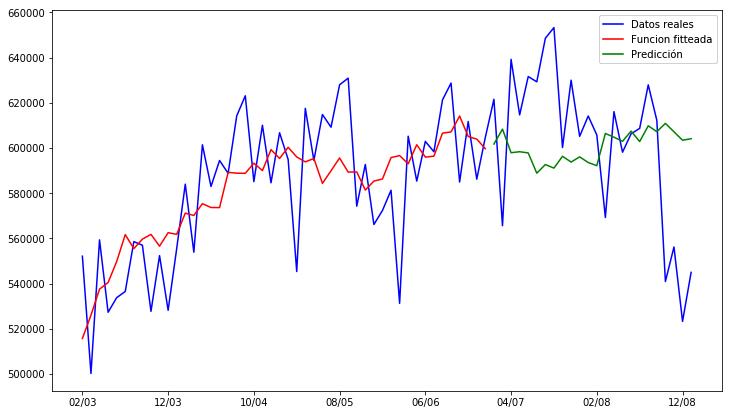
\includegraphics[scale=0.9,natwidth=732,natheight=300]{vuelos_3-6_7-8.png}
\caption{caption}
\label{vuelos-1}
\end{center}
\end{figure}

El error cuadrático medio para estas estimaciones fue de 840810926.93.

Luego se experimentó tomando distintos rangos de entrenamiento: 2003-2005, 2004-2006 y 2005-2007, prediciendo 2005-2006, 2006-2007 y 2007-2008, respectivamente.

\begin{figure}[!htb]
\begin{center}
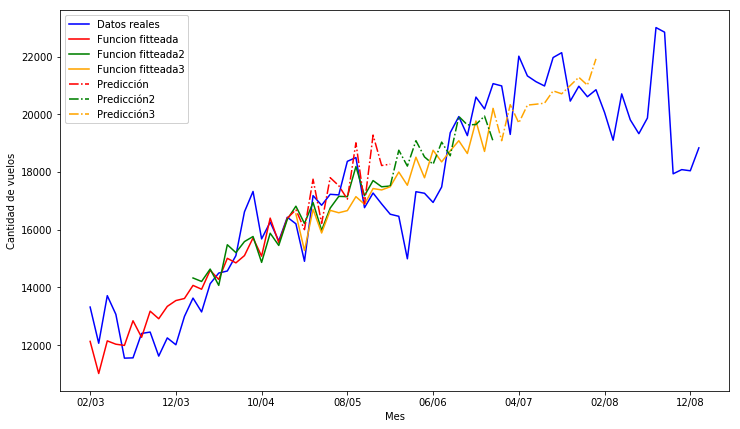
\includegraphics[scale=0.9,natwidth=732,natheight=300]{vuelos_multiples.png}
\caption{caption}
\label{vuelos-2}
\end{center}
\end{figure}

Los EMC fueron 11228017738.2, 1215421229.42, 1214577235.23, según el orden en que los rangos están dispuestos.

Como puede observarse, el EMC para la función entrenada desde 2003 a 2006 es mucho menor que el resto, y esto se cree que se debe a ese año extra que tiene de entrenamiento.


\subsection{ECM de funciones de predicción}

Otra experimentación realizada fue la comparación de los ECM entre distintas funciones de predicción. Se crearon 6 funciones distintas listadas a continuación, de las cuales una es una función lineal y las otras pertenecen a la familia de funciones trigonométricas.

En todas las funciones que corresponden, las letras entre \textit{a} y \textit{l} fueron los parametros que se ajustaron con el entrenamiento, el cual fue dado con la información de los años 2003 a 2006 y luego se procedió a predecir los años 2007 y 2008.

\begin{enumerate}
  \item $y(x) = a + bx$
  \item $y(x) = ax + b|cos(x)| + c|sin(x)| + f  \times  cos(x) + g  \times  sin(x) + d  \times  log(x+1) + e$
  \item $y(x) = hx^4 + ix^3 + jx^2 + ax + b|cos(x)| + c|sin(x)| + f  \times  cos(x) + g  \times  sin(x) + d  \times  log(x+1) + e$
  \item $y(x) = ax + b|cos(x)| + c|sin(x)| + f  \times  cos(x) + g  \times  sin(x) + d  \times  log(x+1) + e + k  \times  sin(x) ^ 2 + l  \times  cos(x) ^ 2$
  \item $y(x) = ax + b|cos(x)| + c|sin(x)| + f  \times  cos(x) + g  \times  sin(x) + d  \times  cos(x) + i  \times  sin(x)  + e$
  \item $y(x) = a + bx + c  \times  cos(xd + e) + f  \times  sin(xg + h) + c  \times  cos(xd + e) + f  \times  sin(xg + h)$
\end{enumerate}


Como hipótesis de este experimento se planteó que la función lineal (1) sería la que mayor error cuadrático medio tendría ya que es la que menor cantidad de parámetros tiene y además es poco flexlible. Dado que las otras 5 funciones pertenecen a la misma familia de funciones, se esperó que éstas tengan un comportamiento similar.

Una vez ejecutado las pruebas, los errores que se obtuvieron para cada función fueron los siguientes:

\begin{figure}[!htb]
\begin{center}
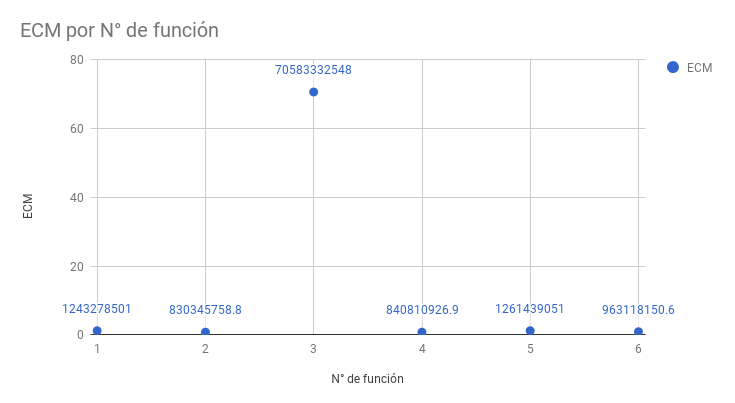
\includegraphics[scale=0.7,natwidth=403,natheight=300]{imagenes/ecm_por_fn.png}
\caption{caption}
\label{vuelos-3}
\end{center}
\end{figure}

Se pudo observar con el anterior gráfico cómo la función número 3 fue la que mayor error cuadrático medio obtuvo y por mucha diferencia a pesar de ser de la misma familia de funciones que las demás (sin contar la función lineal) y de tener la misma cantidad de parámetros que la función número 5. También se observó que la función lineal a pesar de estar muy por debajo que la función 3, estuvo solo un poco por debajo que la función 5 y aun así se mantuvo por encima de las otras 3 funciones.
La función que menor ECM obtuvo fue la función número 4, la cual fue la que mayor cantidad de parametros ajustables tenía.
